\section{Requirements for a practical planner}
The role of the motion planner is to select a sequence of primitives which are dynamically feasible and enable the robot to traverse across the terrain between its start and end point. In general, ensuring dynamic feasibility of a trajectory for an underactuated system requires complicated computations, solving multivariate nonlinear differential equations. Fortunately, as discussed in Section \ref{sec:hzd}, using virtual constraints as motion primitives simplifies the zero dynamics to a function of a single variable and simplifies evaluating dynamic feasibility to a trivial verification of the initial velocity exceeding a lower limit.

As a result, the practical requirements on the motion planner are to ensure that at all chosen primitives are feasible. We recursively define a feasible primitive as one which matches the terrain, has a velocity enabling it to be completed, and is able to be followed by a feasible primitive. Note that this is, in theory, infinitely recursive. In practice, the evaluation of feasibility of a primitive must be limited to a finite step look-ahead. There is typically a requirement on the minimum and the maximum initial velocity of the virtual constraint: the velocity must be sufficient to pass the critical point of the primitive, $\dot{\theta}^c \geq \dot{\theta}_a$, but it also must be low enough that when the swing foot strikes the ground, it does not bounce or slip, $\dot{\theta}^+ \leq \dot{\theta}_b$.

For a useful robot, the initial and final conditions should be at some statically stable resting configuration, however for the purposes of this body of work, it is assumed that the robot begins with some non-zero velocity conducive to dynamically stable walking and need never come to rest. That is, the motion planner is not concerned with the practical considerations of starting or ceasing motion.

Aside from the essential functional requirement of choosing dynamically feasible sequences of primitives, the performance requirements on the planner are quite stringent. Since the objective of this approach is to allow for real-time reactive planning of walking, it is essential that the planner is capable of producing a planned sequence of footsteps in a time span shorter than that taken by the shortest footstep. Note that it is likely that a physical implementation would be in a low-power embedded system which executes software alongside the planner. Clearly, computational efficiency is a large priority for the planning algorithm. This is no surprise, since the motivation for using the virtual constraints method itself is largely in service of reducing on-line computational requirements.

\section{Execution context}
The motion planning algorithm is executed using an iterative receding finite horizon approach. This means that the planner produces a dynamically feasible sequence of some set number of footsteps ahead of the current position, but re-evaluates the sequence significantly earlier than the end-point. This can be considered a form of model-predictive control \cite{camacho2013model}.

For convenience of implementation, we may assume that the planner completes an execution once per footstep. In principle, without disturbances, the planner could execute in a purely feed-forward manner. That is, the path would only be recalculated once the robot reached the endpoint of the previously calculated sequence of primitives. In practice, this is typically not possible; the dynamical model, particularly about impacts, is not a full realisation of the physical system. In addition, it is a very useful property for a planner to produce self-correcting trajectories. Indeed, the planning need not be limited to a single evaluation per footstep. However, assuming disturbances are significantly managed by the controller, it should be sufficient.

The planner requires the initial state $q,\dot{q}$ of the robot, along with an accurate map of the terrain ahead. The necessity of state sensing is unavoidable, both in the planning and control of the robot. However, the sensing requirements of underactuated walkers should not be as intensive as for fully actuated robots due to deferring control of the state evolution to the zero dynamics \cite{collins2005efficient}. The practice of using sensor data to build a terrain map is well-studied, with advancements in the field moving well beyond simple shape mapping to classification \cite{herbert1989terrain, triebel2006multi, brooks2007self}. The algorithm proposed is largely independent of the method used to build the map, whether by prior mapping or real-time scanning, so long as the range of known terrain extends far enough to allow for the chosen number of footsteps ahead to be planned.

\section{Greedy best-first search algorithm}
Manchester \& Umenberger \cite{manchester13planning} present a greedy Best-First Search algorithm capable of producing a dynamically feasible sequence of $k$ motion primitives from the library $L$ which consists of primitives indexed by step lengths $x_f\in X_f$. This algorithm, somewhat modified in order to suit the generated library from Chapter \ref{chap:vclib} and to improve the best-case running time, is presented in Algorithm \ref{alg:bestfirstsearch}. 

\begin{algorithm}
	\begin{algorithmic}[1]
		\Function {BestFirstSearch}{$L,q,\dot{q},\sigma(x),x,k$}
			\State $q_{\mathrm{ind}} \gets$ \Call{impactCondSearch}{$L,q$}
			\State [$p$, success]$\gets$ \Call{AddNode}{$L,q_{\mathrm{ind}},\dot{q},\sigma(x),x,k$}
			\If {success}
				\State MotionControl $\gets p$
			\Else
				\State \Return fail
			\EndIf
		\EndFunction
		\Function {AddNode}{$L,q_{\mathrm{ind}},\dot{q},\sigma(x),x,k$}
			\State $\dot{\theta}_0 \gets \left(c\dot{q}\right)^2$
			\ForAll {$x_f\in X_f$}
				\State $h \gets$ \Call{height}{$\sigma(x),x+x_f$}
				\State $p(x_f) \gets$ \Call{searchLibrary}{$L,q_{ind},s_l,s_h,\dot{\theta}_a$}
			\EndFor
			\While {true}
				\ForAll {$x_f \in X_f$}
					\State $\dot{\theta}^-(x_f) \gets \Gamma_{p(x_f)}(\theta^-)\dot{\theta}_0 + \Psi_{p(x_f)}(\theta^-)$
					\If {$\dot{\theta}^-(x_f) \leq \dot{\theta}_b^2$}
						\State $\dot{\theta}^c(x_f) \gets \Gamma_{p(x_f)}(\theta^c)\dot{\theta}_0 + \Psi_{p(x_f)}(\theta^c)$
					\Else
						\State $\dot{\theta}^c(x_f) \gets \infty$
						\State $[p(x_f),end] \gets$ \Call{nextBest}{$p(x_f)$}
					\EndIf
				\EndFor
				\State $[\dot{\theta}^c,I] \gets$ \Call{sort}{$\dot{\theta}^c$}
				\State $X_f' = X_f(I)$ \Comment{Order the primitives by $\dot{\theta}^c$}
				\ForAll{$x_f \in X_f'$ where $\dot{\theta}^c(x_f)\neq\infty$}
					\If {$k=1$}
						\State \Return {$[p(x_f), \mathrm{success}]$}
					\ElsIf {\Call{aboveGround}{$p(x_f)$}}
						\State $q^+_{\mathrm{ind}} \gets p(x_f).q^+$
						\State $\dot{q}^+ \gets R\Delta\left(\Phi_{p(x_f)}(\theta^+)\right)\Phi_{p(x_f)}'(\theta^+)\sqrt{\Gamma_{p(x_f)}(\theta^+)\dot{\theta}_0 + \Psi_{p(x_f)}(\theta^+)}$
						\State $x^+ \gets x + x_f$
						\State success $\gets$ \Call{AddNode}{$L,q^+_{\mathrm{ind}},\dot{q}^+,\sigma(x),x,k-1$}
						\If {success}
							\State \Return [$p(x_f)$, success]
						\EndIf
					\EndIf
					\State $[p(x_f),end] \gets$ \Call{nextBest}{$p(x_f)$}
				\EndFor
				\If {$\forall x_f\in X_f, end=true$}
					\State \Return fail
				\EndIf
			\EndWhile
		\EndFunction
	\end{algorithmic}
	\caption{Best-first search planning algorithm}
	\label{alg:bestfirstsearch}
\end{algorithm}

\begin{figure}
	\centering
	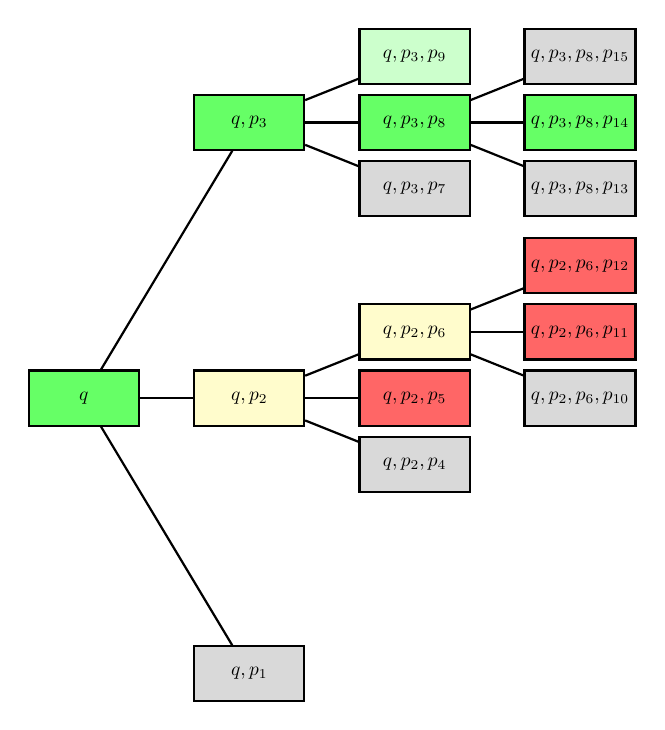
\begin{tikzpicture}[
	scale = 0.7, transform shape, thick,
	every node/.style = {draw, rectangle, minimum width=2cm, minimum height=1cm},
	grow = right,  % alignment of characters
	level 1/.style = {sibling distance=5cm},
	level 2/.style = {sibling distance=1.2cm}, 
	level 3/.style = {sibling distance=1.2cm}, 
	feas/.style={fill=green!60},
	pfeas/.style={fill=green!20},
	qfeas/.style={fill=yellow!20},
	infeas/.style={fill=red!60},
	unch/.style={fill = gray!30},
	level distance = 3cm
	]
	
	\begin{scope}
	\node[feas] {$q$} 
	child { node [unch] {$q, p_1$}}
	child { node [qfeas] {$q , p_2$}
		child {   node [unch] {$q , p_2 , p_4$} }
		child {   node [infeas] {$q , p_2 , p_5$} }
		child {   node [qfeas] {$q , p_2 , p_6$}
			child { node [unch]  {$q , p_2 , p_6 , p_{10}$}}
			child { node [infeas]  {$q , p_2 , p_6 , p_{11}$}}
			child { node [infeas]  {$q , p_2 , p_6 , p_{12}$}}
		}
	}
	child { node[feas] {$q,p_3$}
		child {   node [unch] {$q,p_3,p_7$} }
		child {   node [feas] {$q,p_3,p_8$}
			child { node [unch]  {$q,p_3,p_8,p_{13}$}}
			child { node [feas]  {$q,p_3,p_8,p_{14}$}}
			child { node [unch]  {$q,p_3,p_8,p_{15}$}}
		}
		child {   node [pfeas] {$q,p_3,p_9$} }
	};
	\end{scope}
	\end{tikzpicture}
	\caption[Example decision tree showing a possible traversal of the decision algorithm]{Example decision tree showing a possible traversal of the decision algorithm for a three step lookahead. Solid green indicates a the feasible path found by the algorithm, light green indicates a partial evaluation of feasibility, yellow indicates steps which were feasible themselves but not able to be followed by sufficient feasible footsteps and red indicates infeasible footsteps. Grey nodes were not evaluated.}
	\label{fig:deciontree}
\end{figure}

Figure \ref{fig:deciontree} shows an example of a possible traversal of the path planning algorithm through the decision tree. The algorithm starts with a particular initial configuration $q$ and attempts to build a sequence of $k$ feasible steps. The first task is to find the configuration in the library which best matches $q$ (L2). The algorithm then invokes \textsc{AddNode} with the $k$-step lookahead (L3). The first task is to produce the set of $n_x$ primitives which match the terrain ahead (L12-15). This calls \textsc{SearchLibrary}($L,q_{ind},s_l,s_h,\dot{\theta}_a$) which returns the primitive which has the smallest $\dot{\theta}(\theta^c) \geq \dot{\theta}_a$ in the set of virtual constraints which match the given initial configuration, step length and step height. Note that the \textsc{height} function returns height of the terrain which is quantised such that it corresponds to the values in the library. If this is not possible, e.g. if the height is out of the range of available step heights, the primitive cannot be considered successful for the particular step length $x_f$.

At this point, the algorithm has a decision tree of depth 1. Each of the leaves of the tree corresponds to a virtual constraint which defines a trajectory $q\to q'_i$. Note that at this stage, some of the leaves of the decision tree have been ruled out, since the initial velocity is not sufficient to execute their motions, e.g. $p_1$ in the Figure \ref{fig:deciontree}.

The next step, on L17-25, is to calculate the velocities at the final and critical points. If the final velocity is too large, the primitive is considered infeasible and the \textsc{nextBest} function is called, replacing the primitive with that which has the next smallest $\dot{\theta}(\theta^c)>0$. If there is no such primitive, this function returns $end=true$. This replacement primitive is not considered in this loop iteration, however; the particular step length $x_f$ is associated with $\dot{\theta}^c(x_f) = \infty$.

On L26-27, the primitives are sorted by $\dot{\theta}^c$. At this point, $\dot{\theta}^c > 0$ by design, so the algorithm iterates through the sorted set (L28-41), attempting to find the smallest $\dot{\theta}^c$ which results in a feasible sequence of $k$ footsteps. This involves checking for the primitive's kinematic feasibility (L31) and calling \textsc{AddNode} with $k$ decremented.

In the example decision tree, $p_2$ is found to be a feasible footstep in terms of its velocity, so the algorithm attempts to produce a set of 2 virtual constraints to follow it. $p_4$ is not evaluated due to having insufficient initial velocity and $p_5$ is found to intersect with the ground, but $p_6$ is feasible. However, upon checking for a primitive to follow $p_6$, no feasible footsteps are found. The algorithm returns back to the outermost recursion and through a similar process finds a feasible sequence of primitives $p_3\to p_8 \to p_{14}$. Note that $p_9$ is partially evaluated for feasibility (L18-20) but is not checked further since a feasible path is found.

The incremental improvements made to the algorithm as presented in \cite{manchester13planning} are catalogued below:
\begin{itemize}
	\item The algorithm was modified to take advantage of the pointers stored in the virtual constraint library to the post-impact configuration following the execution of the primitive, availing a $\mathcal{O}(1)$ search for the following initial configuration.
	\item L28-41 was converted from an if statement to a for loop to avoid redundant recalculation of the velocities at the critical and final points. This requires a sort of the primitives by $\dot{\theta}^c(x_f)$. This increases the complexity of that step from $\mathcal{O}(n_x)$ (finding the minimum) to $\mathcal{O}(n_x\log n_x)$. However, it reduces the worst-case number of while loop iterations for single footstep evaluation from $\mathcal{O}(n_xn_qn_k)$ to $\mathcal{O}(n_qn_k)$.
	\item Evaluating the virtual constraint's kinematic feasibility was deferred to L31, where before it was evaluated along with the velocities. This improves the best-case running time since it avoids redundant evaluations.
	\item The calculation of $\dot{\theta}_0^2$ (L11) is completed only once, rather than within the while loop. This is possible because it is independent of the particular virtual constraints, so long as they all synchronise the coordinates in the same manner. This is true of the virtual constraint library generated by the method presented in this thesis.
\end{itemize}

\section[Energy-based heuristic]{Improvements using an energy-based heuristic} \label{sec:heuristic}
Using heuristic methods can direct the decision tree traversal to avoid primitives which will evaluate as infeasible and to guide the search toward sequences of primitives which are more optimal by some measure. It is important to note that the best-first search does not find an optimising sequence; rather it terminates at the first encountered feasible set of primitives. A well-designed heuristic method therefore offers a significant improvement to the algorithm without requiring the structure to be substantially altered.

In \cite{manchester13planning}, an energy-based heuristic is demonstrated to provide significant reductions in traversals through the decision tree. This heuristic involves a simple look-ahead to detect any increases in step height, and acts to add kinetic energy in the lead-up to the change in terrain. This is effective for the specific example of terrain which has a single step-up but has no proven effectiveness for more varied terrain. In particular, it ignores intermediate steps down in the terrain.

An improved energy heuristic is proposed as follows: Model the walker as a point mass a fixed height above the terrain and evaluate the change in gravitational potential energy between the initial position of the robot and a point $kx_m$ in front, where $x_m$ is the maximum step length. Over a course grid, evaluate the relative GPE to the initial point. From this, we can evaluate the required kinetic energy additions and subtractions to maintain the velocity of the robot within set bounds.
	
One would not expect this heuristic to be significantly more efficacious than that which was previously proposed. However, it should prove better at directing the search towards the least wasteful primitives, improving the overall efficiency of the robot. In addition, and perhaps more importantly, this method should not direct the algorithm towards primitives which will exceed the maximum velocity for the robot when seeing steps up in the distance with more immediate steps down. Examining the merits of this proposed heuristic are deferred to a later work, since the robot model used in the verification of the library generation method is too simple to allow for traversal over very rough terrain, which would appear to be the only use case where it may be necessary to use the improved heuristic over that already tested in \cite{manchester13planning}.

\section{Complexity analysis} \label{sec:complexity}
The time complexity of the algorithm is based upon the contribution of the search through the library of primitives for each given $q^+,s_l,s_h$ triple, the number of searches per footstep, and the number of steps $k$ in the decision tree. Note that at each footstep, the number of searches into the library is $n_x$.

Before the first invocation of \textsc{AddNode}, it is necessary to find the initial configuration $q^+$ in the list of impact configurations $\tilde{Q}$. This is completed in $\mathcal{O}(|\tilde{Q}|)=\mathcal{O}(\log(n_xn_yn_q))$ time. Every subsequent call to \textsc{AddNode} is completed with a pointer into $\tilde{Q}$, making the search time for the initial configuration of all succeeding steps $\mathcal{O}(1)$.

Each time the library is searched with a given $q^+,s_l$ and $s_h$, the particular step height must be found in the set of heights (L12-15). Since the heights are ordered, this is completed in $\mathcal{O}(\log n_y)$. After this search, at the leaf, the algorithm searches for the constraint with velocity closest to $\dot{\theta}_a$. If this is the velocity for which the ordering was calculated, the algorithm may use a binary search, thus the complexity is $\mathcal{O}(\log(n_qn_k))$, resulting in a total complexity for the library search of $\mathcal{O}(\log n_y+\log(n_qn_k))$ However, if the desired $\dot{\theta}_a$ is not the velocity on which the sort was calculated and the set of virtual constraints is not subject to a velocity-independent ordering, the complexity is $\mathcal{O}(\log n_y +n_qn_k)$.

Once a set of virtual constraints has been selected, they are ordered by velocity. This is a $\mathcal{O}(n_x\log(n_x))$ operation. The rest of the in-loop calculations are not dependent on any of the size variables, thus are completed in $\mathcal{O}(1)$ time. However, the for loops on L17-L25 and L28-L41 complete $n_x$ times per iteration of the outer while loop (L16-45).

It is instructive here to consider the worst-case and best-case running times of the algorithm, since the termination occurs when a feasible path is found, which leads to a significant difference in these two cases. In practice, so long as the terrain is passable by the robot, the running time should be close to best-case, particularly when guided by a heuristic.

The worst-case running time occurs when no feasible steps are found but this is only detected at the $k$th step each time and all virtual constraints in the library are feasible up until this point. In this case, the algorithm performs a complete search over every virtual constraint in the library which is applicable to the terrain, over $k$ footstep evaluations. This results in $n_qn_k$ outer loop iterations per footstep evaluation, and an exponential complexity in the number of footsteps. Therefore the worst-case time complexity $T_w$ is
\begin{align*}
	T_w &\in \mathcal{O}\left(|\tilde{Q}| + (S + L)^k\right) \\
	S &= n_x(\log n_y + \log(n_qn_k)) \\
	L &= n_qn_k(n_x + n_x\log n_x) \\
	\therefore T_w &\in \mathcal{O}\left(\log(n_xn_yn_q)+(n_x(\log n_x + \log n_y + n_qn_k))^k\right)
\end{align*}
Note that in this case, the ordering method does not assist in the running time of the algorithm. This makes sense, since the worst case occurs when the first element in every set of virtual constraints is feasible.

The best-case running time occurs when the first feasible footstep results in a feasible set of successors at each step up to the $k$th. In this case, the algorithm completes only a single iteration of the outer loop and second for loop at each footstep. Therefore, the best-case running time is
\begin{align*}
	T_b &\in \mathcal{O}\left(|\tilde{Q}| + k(S + L')\right) \\
	L' &= n_x + n_x\log n_x \\
	\therefore T_b &\in \mathcal{O}\left(\log(n_xn_yn_q)+kn_x(\log n_x + \log n_y + \log(n_qn_k))\right)
\end{align*}
If the ordering is not used, this becomes
\[
T_b \in \mathcal{O}\left(\log(n_xn_yn_q)+kn_x(\log n_x + \log n_y + n_qn_k)\right)
\]

It is reasonable to believe that the running time of the algorithm is much more likely to be near $T_b$ than $T_w$, since the worst case for this algorithm requires quite a contrivance. It is difficult to imagine how all of the virtual constraints in the library could be feasible up to $k-1$ footsteps, but then every one infeasible at the $k$th step, for a rich and practicable library.

It ought to be noted that despite the reasonably complicated appearance of $T_b$, the best-case running time of the algorithm is very fast, logarithmic in all of the dimensions of the library other than $n_x$, where it is log-linear, and linear in $k$. Additionally, recall that $n_x$ is kept small by design. Since the kinematic and dynamic feasibility of an individual virtual constraint is able to be verified very rapidly, this algorithm should, at least in the best case, be able to traverse very large libraries in real-time on a low-powered system with a reasonable step look-ahead.